\documentclass[pdflatex,compress]{beamer}

%\usetheme[darktitle,framenumber,totalframenumber]{UA}
\usetheme[dark,framenumber,totalframenumber]{UA}
% \setbeamertemplate{background}[grid][step=1cm]
% \beamertemplategridbackground{1}

\usepackage{subcaption}
\usepackage{fontspec,microtype}
\usepackage{unicode-math}
\defaultfontfeatures{Ligatures=TeX, Scale=MatchLowercase, Numbers=Lining}
\graphicspath{{figs/}}

\setmainfont[
BoldFont=texgyreheros-bold.otf,
ItalicFont=texgyreheros-italic.otf,
BoldItalicFont=texgyreheros-bolditalic.otf,
]{texgyreheros-regular.otf}
\setsansfont[
BoldFont=texgyreheros-bold.otf,
ItalicFont=texgyreheros-italic.otf,
BoldItalicFont=texgyreheros-bolditalic.otf,
]{texgyreheros-regular.otf}


\title{Let's Get Talking}
\subtitle{Speech Recognition for \\Low-Resourced\\Languages}

\author{Joshua Meyer}

\begin{document}

% ----------------------------------------------------------------------------
% *** Titlepage <<<
% ----------------------------------------------------------------------------
\maketitle
% ----------------------------------------------------------------------------
% *** END of Titlepage >>>
% ----------------------------------------------------------------------------


% ----------------------------------------------------------------------------
% ----------------------------------------------------------------------------


\begin{frame}
  \frametitle{}
  \centering
  \begin{center}
    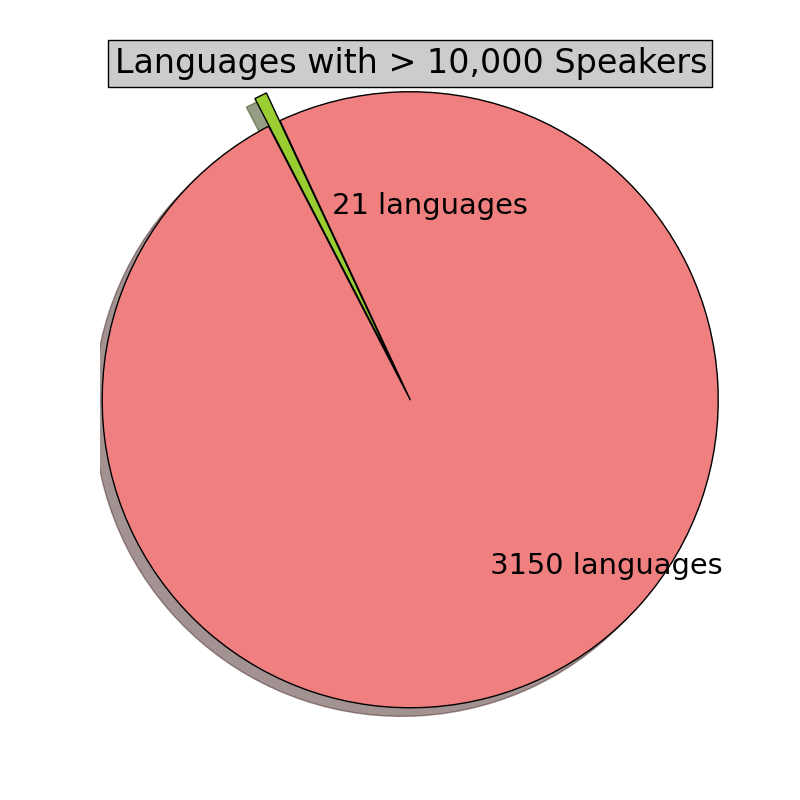
\includegraphics[width=\textwidth,height=0.8\textheight,keepaspectratio]{siri.png}
  \end{center}
\end{frame}

\begin{frame}
  \frametitle{}
  \centering
  \begin{center}
    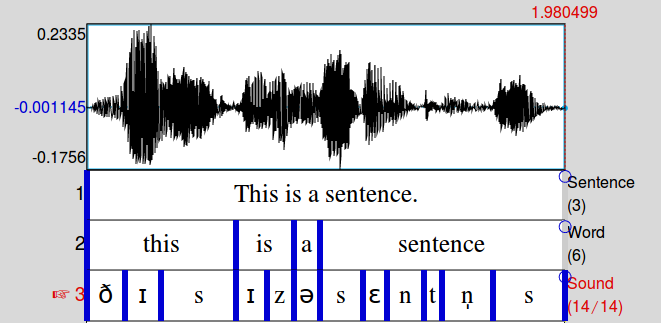
\includegraphics[width=\textwidth,height=0.8\textheight,keepaspectratio]{sentence.png}
  \end{center}
\end{frame}

\begin{frame}
  \frametitle{}
  \centering
  \begin{center}
    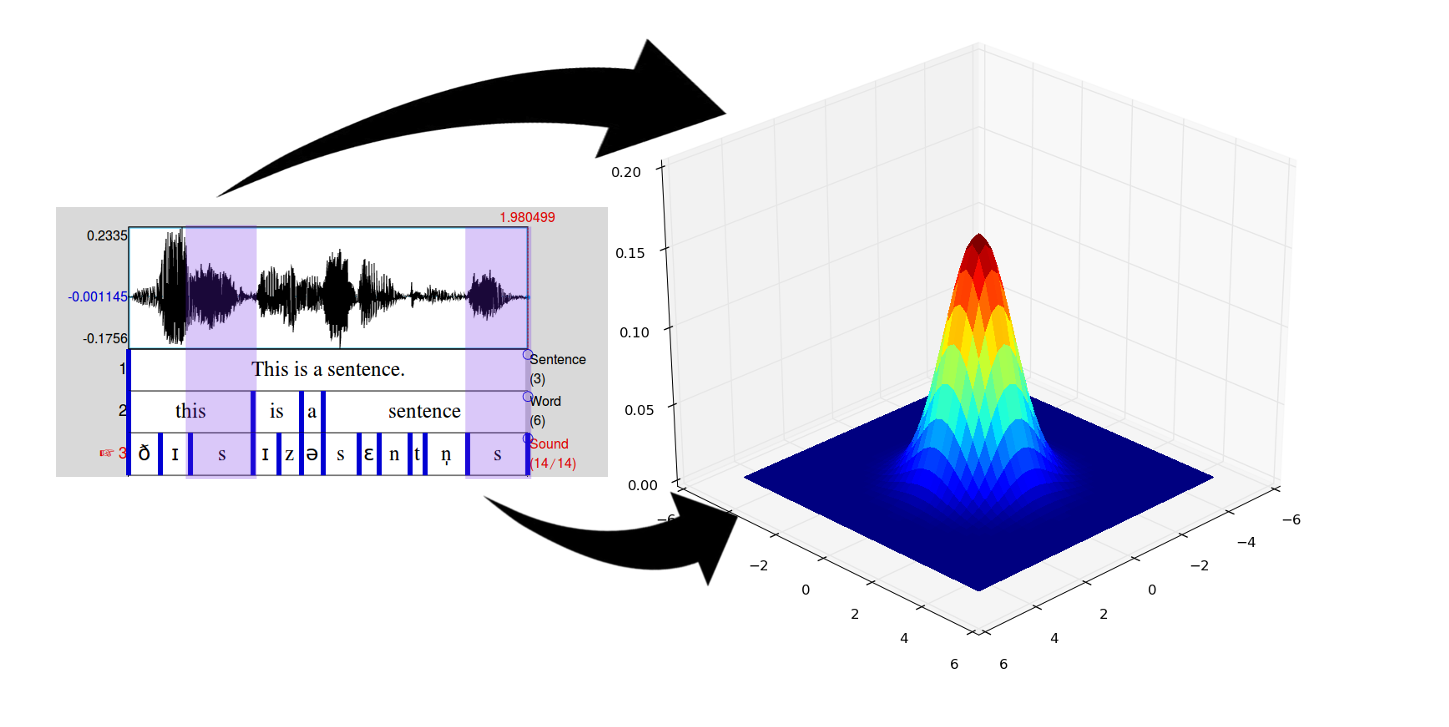
\includegraphics[width=\textwidth,height=0.8\textheight,keepaspectratio]{extraction.png}
  \end{center}
\end{frame}


\begin{frame}
  \frametitle{}
  \centering
  \begin{center}
    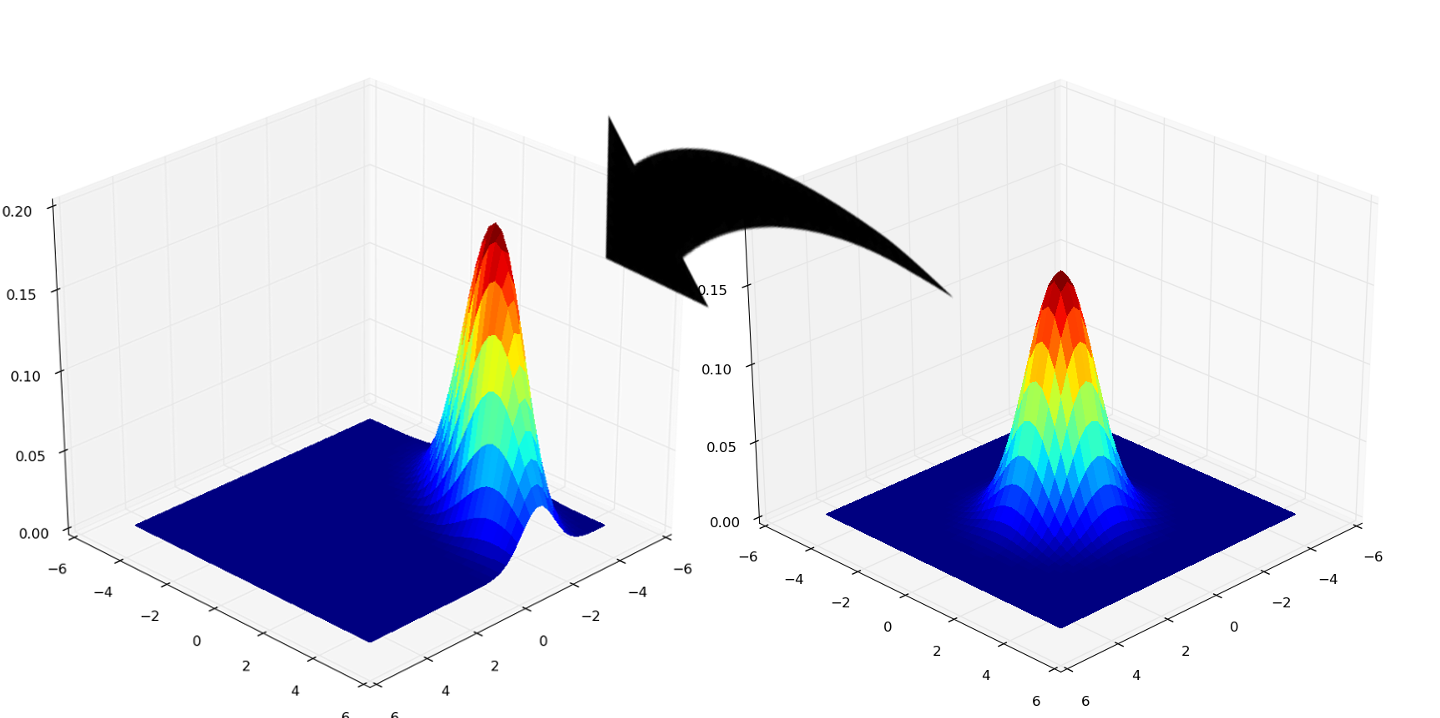
\includegraphics[width=\textwidth,height=0.8\textheight,keepaspectratio]{adaptation.png}
  \end{center}
\end{frame}

\begin{frame}
  \frametitle{}
  \begin{center}
    \Huge{Thank you!}\\
    \vspace{1cm}
    
\includegraphics[width=\textwidth,height=0.25\textheight,keepaspectratio]{nsf-trans.png}
  \end{center}
\end{frame}


% ----------------------------------------------------------------------------
% ----------------------------------------------------------------------------


\end{document}
